\subsection{Process}

\begin{theorem}{(61)} Process control block (PCB):\begin{itemize}
        \item Process ID.
        \item Prcoess state.
        \item CPU register (stack top pointer, accumulator).
        \item Program Counter (PC).
        \item CPU scheduling info (PCB pointer, process priority).
        \item Memory management info (base/limit registers, page table).
        \item Accounting info (CPU time).
        \item I/O-status info (Uncompleted I/O request, allocated I/O devices).
    \end{itemize}
\end{theorem}

\begin{theorem}{(60, 61)} Process life cycles (Figure \ref{img:process_lifecycles}): \begin{itemize}
        \item State:\begin{itemize}
            \item New (Created):Process is created and PCB is allocated in kernel, but memory space is NOT allocated.
            \item Ready:Prcoess is allocated memory space, being put in ready queue. Ready for execution, being able to get CPU allocation.
            \item Waiting (Block, Sleep in memory):Waiting for some event to occur, being put in waiting queue, e.g. waiting for I/O-completed. Unable to get CPU allocation.
            \item Terminated (Exit, Zombie):Process is finished.
        \end{itemize}
        \item Transition:\begin{itemize}
            \item Admitted:Prcoess is allocated memory space. In batch system, use long-term scheduler to decide which process to load into memory. In time-sharing and real-time systems, do NOT use long-term scheduler.
            \item Dispatch:Short-term (CPU) scheduler decides which process to get CPU allocation and allocates CPU to execute.
            \item Exit:Process is finished, releasing resources.
            \item Interrupt (Time-out):Process release CPU, putting on ready queue, e.g. time-out interrupt.
            \item I/O event wait:Process waits for I/O-completed or event occurs.
            \item I/O-completed or event occurs:I/O-completed or event occurs, putting in ready queue.
            \item Only in Stalling version (Figure \ref{img:process_lifecycles_stalling}):\begin{itemize}
                \item Swap out:Out of memory, and other process needs more space. Medium-term scheduler can choose some \textbf{Blocked} processes to swap out to disk with their process image being saved.
                \item Swap in:Sufficient memory space. Medium-term scheduler can choose some Suspended/Ready processed to swap in from disk to memory, putting in ready state.
                \item Suspend:Out of memory even all Blocked processes are swapped out or Blocked processes got higher priority than Ready processes. Swap out some \textbf{Ready} processes to get sufficient memory space.
                \item (Poor design) Running to Suspended/Ready:If a higher priority Suspended/Block process becomes Ready, kernel can force a lower priority Running process to release CPU and memory space, putting the former in running queue.
                \item (Poor design) Suspended/Block to Suspended/Ready:If as Suspended/Blocked got higher priority than a Running process, the latter release CPU and memory space, swapping in the former and get CPU allocation.
            \end{itemize}
        \end{itemize}
        \item Zombie state:Process is finished, but the parent process have NOT collected results of the children processes, or parent process have NOT executed wait() system call. Resources are released, but PCB have NOT been deleted, until parent process collects the results, then kernel delete PCB.
    \end{itemize}
\end{theorem}

\begin{figure}[H]
    \centering
    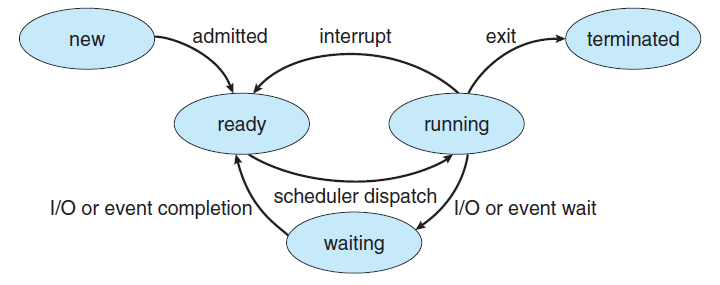
\includegraphics[scale=0.8]{img/process_lifecycles.png}
    \caption{Process life cycles.}
    \label{img:process_lifecycles}
\end{figure}

\begin{figure}[H]
    \centering
    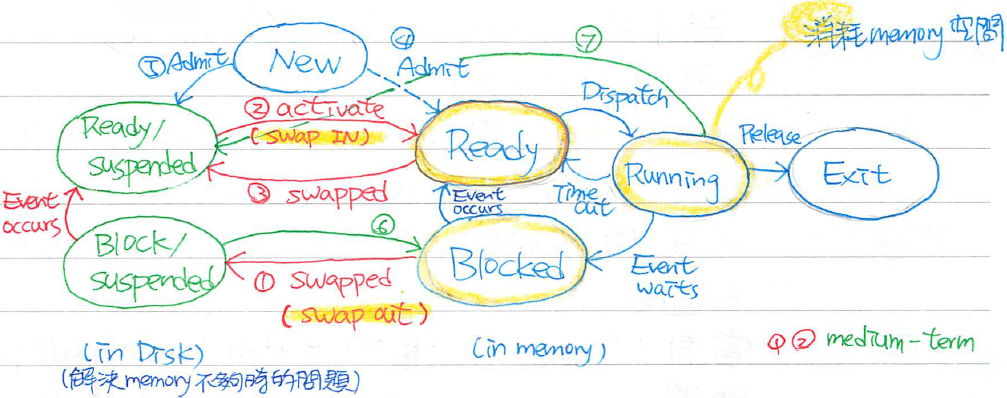
\includegraphics[scale=0.75]{img/process_lifecycles_stalling.png}
    \caption{Process life cycles (Stalling version).}
    \label{img:process_lifecycles_stalling}
\end{figure}

\subsection{Scheduling}

\begin{theorem}{(67)} Scheduler:\begin{itemize}
        \item Long-term (Job) scheduler:通常batch system採用,time-sharing與real-time systems不採用,從job queue中選jobs載入memory。執行頻率最低,可以調控multiprogramming degree與CPU-bound與I/O-bound jobs的比例。
        \item Short-term (CPU, process) scheduler:從ready queue選擇\textbf{一個}process分派給CPU執行。所有系統都需要,執行頻率最高,\textbf{無法}調控multiprogramming degree與CPU-bound與I/O-bound jobs的比例。
        \item Medium-term scheduler:Memory space不足且有其他processes需要更多memory時執行,選擇Blocked或lower priority process swap out to disk。Time-sharing system採用,batch和real-time systems不採用,可以調控multiprogramming degree與CPU-bound與I/O-bound jobs的比例。
    \end{itemize}
\end{theorem}

\begin{theorem}{(69, 70)} \quad\quad \begin{itemize}
        \item Context switch:\begin{itemize}
            \item 執行期間無法執行process,主要取決於硬體因素。
            \item 降低負擔:\begin{itemize}
                \item 提供Multiple registers set:每個process有自己的registers set,只需要切換pointer就能context switch。
                \item 使用Multi-threading。
            \end{itemize}
        \end{itemize}
        \item Dispatcher:\begin{itemize}
            \item 將CPU真正分配給CPU scheduler選擇的process。
            \item Context switch.
            \item Switch mode to user mode.
            \item Jump to execution entry of process.
        \end{itemize}
    \end{itemize}
\end{theorem}

\begin{theorem}{(63)} Process control operation: \begin{itemize}
        \item \code{fork()}:\begin{itemize}
            \item child process有與parent process不同的memory space,而起始code section和data section皆來自parent process的複製。
            \item 失敗:回傳負值;成功:回傳$0$給child process,$> 0$值即child process PID給parent process。
        \end{itemize}
        \item \code{wait()}:若child process已終止,帶parent process還沒執行$wait()$,但kernel含不能清除child process PCB,直到parent process收集完child process info,此段期間稱zombie。
        \item \code{execlp(dir, filename, args)}:載入特定工作執行,memory content不再是parent process的複製,沒有參數填\code{NULL},e.g. \code{execlp("/bin/ls", "ls", NULL)}。
    \end{itemize}
\end{theorem}

\begin{theorem}{(70)} 評估scheduling performance: \begin{itemize}
        \item CPU utilization:$\frac{\text{CPU process execution time}}{\text{CPU total time}}$。
        \item Throughput:單位時間完成process數量。
        \item Waiting time:Process在\textbf{ready queue}的時間。
        \item Turnaround:Process進入系統到完成工作的時間。
        \item Response time:user輸入到系統產生第一個回應的時間。
    \end{itemize}
\end{theorem}

\begin{theorem}{(75)} \quad\quad \begin{itemize}
        \item Starvation:\begin{itemize}
            \item Process長期無法取得完成工作所需資源,因此遲遲無法完成,形成indefinite blocking。
            \item 容易發生在不公平或是preemptive的scheduling。
            \item 有機會完成但是機會很小。
            \item 通過Aging解決:當process在系統中時間增加,逐漸提升process的prioirty。但是soft real-time systems不能使用Aging,因為會違反定義。
        \end{itemize}
        \item Non-preemptive (Cooperative):\begin{itemize}
            \item 完成工作時間較可預期。
            \item Context switch次數較少。
            \item 較少發生Race condition,特別是kernel。
            \item Scheduling performance較差,平均等待時間較長。
            \item Real-time和time-sharing systems不適合。
        \end{itemize}
        \item Preemptive:\begin{itemize}
            \item 大部分OS在kernel mode採用,防止race condition。
            \item 對soft real-time systems不利,例如kernel執行時
        \end{itemize}
    \end{itemize}
\end{theorem}

\subsubsection{Scheduling algorithms}

\begin{theorem}{(71, 72, 75, 76, 77, 78)} Scheduling algorithms: \begin{itemize}
        \item FCFS (First-come-first-serve):可能遭遇Convoy effect,即許多processes都在等待一個需要很長CPU time的process完成工作。
        \item SJF (Shortest-Job-First):\begin{itemize}
            \item Preemptive SJF又稱SRTF (Shortest-Remaining Time First)。
            \item 效益最佳(包含SRTF),即平均等待時間最短。
            \item 對long-burst time job,可能有starvation。
            \item 不適合用在CPU (short-term) scheduling,因為不知道process的精確next CPU burst time,短時間也難以精準預估。
            \item Long-term job可能可行。
            \item Exponential Average:預估next CPU burst time。\begin{equation}
                \tau_{n + 1} = \alpha t_n + (1 - \alpha)\tau_n
            \end{equation} 其中,$t_n$為本次CPU實際值,$\alpha$為機率。
        \end{itemize}
        \item Priority scheduling:FCFS, SJF, SRTF $\subset$ Priority scheduling
        \item Round-Robin (RR) scheduling:\begin{itemize}
            \item Time-sharing system採用。
            \item FCFS $\subset$ RR
            \item 效能取決於time quantum大小,太小context switch太頻繁。
            \item Time quantum大小會影響turnaround time,平均turnaround time\textbf{未必}會隨著quantum time增加而下降。
        \end{itemize}
        \item Multi-level queue:\begin{itemize}
            \item Queue之間採用fixed priority preemptive scheduling或RR。
            \item 每個queue有各自的scheduling。
            \item process不能在queues之間移動,因此缺乏彈性。
            \item 易starvation,且無法通過類似Aging改善。
        \end{itemize}
        \item Multi-level feedback queue:\begin{itemize}
            \item 允許process在queues間移動,可降級增加彈性。
            \item No starvation,可以採用Aging防止starvation。
            \item 所有scheduling superset。
        \end{itemize}
        \item Combination of RR and Priority scheduling:多個processes有相同priority時,採用RR。
        \begin{table}[H]
            \centering
            \begin{tabular}{|c|c|c|c|c|}
                \hline
                Scheduling & 公平 & Preemptive & Non-preemptive & Starvation \\
                \Xhline{2\arrayrulewidth}
                FCFS & $\surd$ & & $\surd$ & \\
                \hline
                SJF & & & $\surd$ & $\surd$ \\
                \hline
                SJF & & $\surd$ & & $\surd$ \\
                \hline
                Priority & & $\surd$ & $\surd$ & $\surd$\\
                \hline
                RR & $\surd$ & $\surd$ & & \\
                \hline
                Multi-level queue & & $\surd$ & & $\surd$ \\
                \hline
                Multi-level feedback queue & & $\surd$ & & \\
                \hline
            \end{tabular}
        \end{table}
    \end{itemize}
\end{theorem}

\subsubsection{特殊系統scheduling}

\begin{theorem}{(79)} Multiprocessors system:\begin{itemize}
        \item 包含多CPUs,Multicores,NUMA system,Heterogeneous(手機上多核CPU)system,Multithreaded(硬體)system。
        \item 多CPUs:\begin{itemize}
            \item ASMP:類似single-CPU scheduling。
            \item SMP:分 2 approaches:\begin{itemize}
                \item 所有CPU共用一條ready queue,no load balancing problem,須防止race condition。
                \item 每一個CPU有各自ready queue,可能有load balancing problem,可以通過kernel協調imbalance CPUs給其他ideal CPUs processes。
            \end{itemize}
        \end{itemize}
        \item Processor affinity:\begin{itemize}
            \item 一但process在某CPU上執行,盡量避免migration。
            \item 因為migration from one CPU to another,first CPU cache should be invalidated and second CPU cache should be repopulated,it cost a lot。
            \item Migrating a process may incur a penalty on NUMA systems, where a process may be moved to a CPU that requires longer memory access time。
        \end{itemize}
        \item Multicores:有Memory stall problem。\begin{itemize}
            \item 通過Multithreaoded processing cores解決,2 or more hardware threads are assigned to each core。
            \item 當一thread memory stall,core can switch to another thread。
            \item 每個thread OS視為logical CPU,皆可執行software thread (process),稱為Cheap Multithreading Technology (CMT)。
        \end{itemize}
    \end{itemize}
\end{theorem}

\begin{theorem}{(80)} Real-time system:\begin{itemize}
        \item Soft real-time system:\begin{itemize}
            \item 採用preemptive和priority scheduling,不提供aging。
            \item Minimize latency:包含interrupt latency和dispatch latency (Figure \ref{img:real_time_dispatch}),real-time system不適合non-preemptive;若是preemptive,須防止race condition。
            \item Prioity inversion:Higher priority process waits for lower priority process to release resources. 通過Priority inheritance解決:讓lower priority process暫時繼承higher priority,以便盡快取得CPU執行,完成後再恢復lower priority。
            \begin{figure}[H]
                \centering
                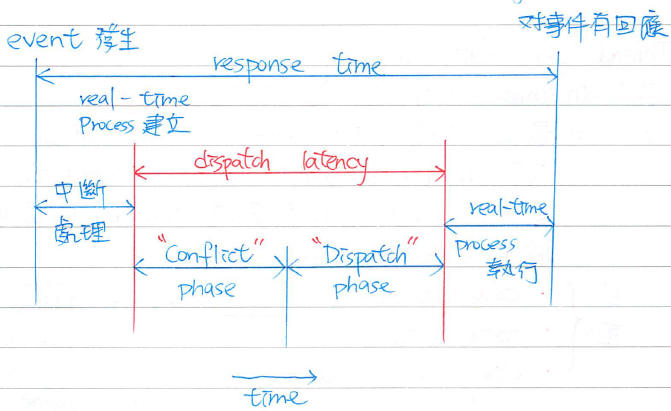
\includegraphics[scale=0.8]{img/real_time_dispatch.png}
                \caption{Dispatch latency on real-time systems.}
                \label{img:real_time_dispatch}
            \end{figure}
        \end{itemize}
    \end{itemize}
\end{theorem}

\begin{theorem}{(80)} Hard real-time system:\begin{itemize}
        \item 討論Synchronous real-time event scheduling,即每隔一段時間發生,需在deadline前完成。
        \item Schedulable判斷:\begin{equation}
            \sum_{i = 1}^{n} \frac{c_i}{p_i} \le 1
        \end{equation} 若符合則schedulable。其中,$n$為事件數目,$c_i$為CPU burst time,$p_i$為period time。
        \item Process meets deadline scheduling algorithms:\begin{itemize}
            \item Rate-Monotonic:\begin{itemize}
                \item Static priority且preemptive。
                \item Period time越小,則priority越高。
                \item Under schedulable,也\textbf{不能}保證所有event皆滿足deadline。
                \item 若其無法滿足deadline,其他static priority scheduling也無法。
            \end{itemize}
            \item EDF:\begin{itemize}
                \item Dynamic priority且preemptive。
                \item Deadline越小,則priority越高。
                \item Under schedulable,保證所有event皆滿足deadline。
                \item CPU utilization不可能達到$100\%$。
            \end{itemize}
        \end{itemize}
    \end{itemize}
\end{theorem}

\subsection{Thread}

\begin{theorem}{(86)} Thread:\begin{itemize}
        \item 又稱Lightweight process。
        \item process是OS分配\textbf{resources}的基本單位,而thread是OS分配\textbf{CPU time}的基本單位。
        \item 每一條thread有private Thread Content Block (TCB),包含PC、registers、stack和local variables等,因此須防止race condition。
        \item 同一process之threads共享process的data section (static local and global variables)、heap和code section等,在同一個address可以有多個threads同時執行。
        \item 若一thread被blocked,則CPU可切換給其他thread執行,所以process不會blocked。
        \item Private contents較traditional prcocess少,context switch較快。
        \item 同一process的不同threads可以平行在不同CPUs上執行。
        \item 種類:\begin{itemize}
            \item User-level thread:\begin{itemize}
                \item 由在user site的thread library管理,不需要kernel管理,e.g. POSIX的pthread library,但只是提供規格並沒有實現。
                \item Kernel不知道其存在,因此kernel不干預,導致不同threads\textbf{無法}平行在不同CPUs上執行。
                \item 若user thread發出blocking system call時,則該process也會被blocked,即時該process還有其他available threads。
            \end{itemize}
            \item Kernel-level thread:現行OS皆支持。
        \end{itemize}
        \item Pthread library is provided by user-level or kernel-level.
        \item Windows Thread library and Java Thread library are kernel-level threads.
    \end{itemize}
\end{theorem}

\begin{theorem}{(88)} Thread model (user thread-to-kernel thread):\begin{itemize}
        \item Many-to-One model:即user-level thread。
        \item One-to-One model:\begin{itemize}
            \item Not efficient than Many-to-One model.
            \item 若建立過多user thread,kernel overhead過重,performance下降,一般會限制thread數量。
            \item e.g. Linux, family of Windows OS, OSX.
        \end{itemize}
        \item Many-to-Many model:\begin{itemize}
            \item Overhead較One-to-One小,但製作較複雜。
            \item Not efficient than Many-to-One model.
            \item e.g. Solaris 2,但它是用two-level mapping model製作,同時也允許One-to-One。
        \end{itemize}
    \end{itemize}
\end{theorem}

\begin{theorem}{(90)} Threading issues:\begin{itemize}
        \item \code{fork()} issue:若parent和child thread工作相同,則複製parent process所有threads到child thread;反之,則只複製該thread到child process。
        \item Signal delivery issue: \begin{itemize}
            \item 種類:\begin{itemize}
                \item Synchronous:自作自受,e.g. Divide-by-zero。
                \item Asynchronous:池魚之殃,e.g. aborted by system admin, parent被終止,child也一同被終止。
            \end{itemize}
            \item Signal delivery:\begin{itemize}
                \item Deliver signal to the thread to which the signal applies, e.g. synchronous signal.
                \item Deliver signals to all threads, e.g. user abortion.
                \item Deliver signals to some threads, e.g. kill.
                \item Assign a specific thread to receive all signals for its process, e.g. Solaris 2. 
            \end{itemize}
        \end{itemize}
    \end{itemize}
\end{theorem}
